\subsection{Rayleigh-Taylor instability}\label{sec:rayleigh}
This problem has been originally presented by \citet{vanKeken1997} and here it is performed as the isoviscous case (Case 1a). The domain has $L_x=0.9142$ and
$L_y=1$ and gravity $\bm{g}=(0,-1)$. Two fluids with same constant viscosities ($\eta_1=\eta_2=1$) and different densities ($\rho_1=1000$ and $\rho_2=1010$),
with the lighter fluid at the bottom. The initial interface between the fluids is given by $y(x)=0.2+0.02 \cos \left(\frac{\pi x}{L_x}\right)$. The experiment
is performed with different grid sizes ($50\times50, 80\times80, 100\times100$ and $256\times256$). A total of 1960000 markers are randomly distributed at the
beginning of the simulation. Velocity boundary conditions are set to no slip at the top and the bottom, and to free slip at the sides of the domain.

$v_{\textrm{rms}}$ as function of time is reported in Fig. \ref{fig:RT}, matching well with results shown by \citet{vanKeken1997}, \citet{Tackley2003} and
\citet{Thieulot2014}. Fig. \ref{fig:rayleigh} shows the evolution of the experiment at different time steps. All data can be found at 
\url{https://github.com/aleregorda/Benchmarks/tree/main/Momentum_equation/Rayleigh_Taylor_experiment/ISOVISCOUS}.

\begin{figure}
\centering
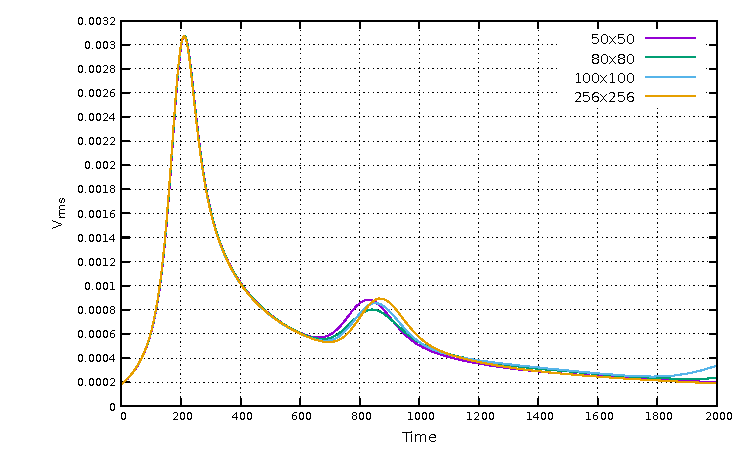
\includegraphics[width=400px]{./Figures/RT.pdf}
\caption{$v_{\textrm{rms}}$ of the Rayleigh-Taylor experiment as function of time for different resolution of the grid.}
\label{fig:RT}
\end{figure}

\begin{figure}
\centering
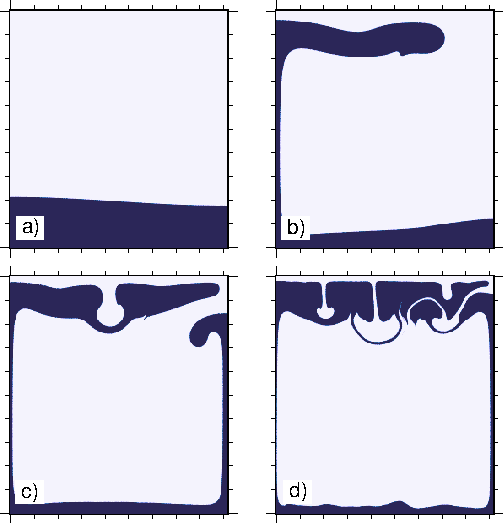
\includegraphics[width=300px]{./Figures/Rayleigh.pdf}
\caption{Evolution of the Rayleigh-Taylor experiment for a grid of $256\times256$ elements at $t=0, 500, 1000$ and $2000$ (panels a, b, c and d, respectively).}
\label{fig:rayleigh}
\end{figure}